\documentclass[9pt,twocolumn,twoside]{gsajnl}
% Use the documentclass option 'lineno' to view line numbers

\articletype{inv} % article type
% {inv} Investigation 
% {gs} Genomic Selection
% {goi} Genetics of Immunity 
% {gos} Genetics of Sex 
% {mp} Multiparental Populations
\usepackage{cite}
\usepackage{url}


\title{New insights of the RNA-seq data of \textit{The Cancer Genome Atlas} for Papillary Thyroid Carcinoma}

\author[$\ast$,1]{Luís Revilla}
\author[$\ast$]{Marina Reixachs}
\author[$\ast$]{Mauro Álvarez}
\author[$\ast$]{Inés Sentís}


\affil[$\ast$]{Universitat Pompeu Fabra}


\keywords{Cancer; Genomics; Thyroid; Differential Expression; RNA-Seq}

\runningtitle{GENETICS | INVESTIGATION} % For use in the footer 

\correspondingauthor{Revilla}

\begin{abstract}
Papillary Thyroid Carcinoma (PTC) is the most common type of thyroid cancer \citep{Agrawal2014a}. It is more prevalent in women than men and its common diagnosis occurs between 25 and 65 years old \citep{tcga}. The aim of our project is to study differentially expressed genes between tumor and normal samples taking into account whether there could be a gender effect on the tumorgenesis of PTC. Using data from the \citet{tcga} we have performed a differential expression analysis. Comparisons were made according to the patients gender and the disease state of the sample (tumor or normal) and revealed that Female-Normal samples have more up-regulated (over-expressed) genes respect to Female-Tumor samples as well as more than to Male-Tumor samples and Male-Normal samples. Functional enrichment performed with GO annotations suggested that tumorgenesis in females might be faster and therefore, more energetically demanding, than males. This sould be a reason why thyroid cancer is more prevalent in females than males. Nevertheless, further investigation must be done so our results should be treated with caution. 

\end{abstract}

\setboolean{displaycopyright}{true}

\begin{document}

\maketitle
\thispagestyle{firststyle}
\marginmark
\firstpagefootnote
\correspondingauthoraffiliation{Universitat Pompeu Fabra. Doctor Aiguader, 80. 08003 Barcelona (Spain). 
Email: lluis.revilla01@estudiant.upf.edu}
\vspace{-11pt}%


\section*{Introduction}

Thyroid cancer can develop from the different cells that form the follicles of the thyroid. This gland located at the base of the throat secretes hormones such as T3 and T4 that have metabolic functionalities such as control of heart rate, blood pressure, body temperature and weight \citep{tcga}.

From the four types of thyroid cancer (papillary, follicular, medullary and anaplastic thyroid cancer) Papillary Thyroid Carcinoma (PTC) is the most common type of thyroid cancer \citep{Agrawal2014a}. It is more prevalent in women than men and its common diagnosis occurs between 25 and 65 years old \citep{risk}.

Driver onco-mutations for this type of cancer appear as alterations of the MAPK signaling pathway and the PI3K-AKT pathway \citep{Kimura2003}. Both are implied in cell proliferation and survival and in human tumorigenesis. The overactivation of the MAPK pathway because of mutations such as the BRAFV600E mutation, leads to the development of PTC from follicular thyroid cells. On the other hand, mutations that activate the PI3K-AKT pathway, such as mutations in RAS, PTEN and PIK3CA, mostly leads to development of Follicular Thyroid Adenoma (FTA) and Follicular Thyroid Cancer (FTC) also in follicular thyroid cells \citep{Xing2013a}.

Research from \citet{tcga} focused on PTC and they found that a part from alterations in BRAF, specifically BRAFV600E, and RAS, there are other driver mutations such the ones in EIF1AX PPM1D and CHEK2 genes that are main alterations for that type of thyroid cancer. They proposed a new classification of PTC subtypes based on their molecular findings. 

The aim of our project deviates from being a replicate of the TCGA project. Our academic purpose has been to study differentially expressed genes from tumor and normal samples but also taking into account whether there could be a gender effect on the tumorgenesis of PTC. To our knowledge, there is no clear reason why thyroid cancer is more prevalent in women than men \citep{intro}. Therefore, it would be interesting to analyze whether there are differentially expressed genes within genders and respect to thyroid cancer. In addition, in case there are significant differences in gene expression which are the potential biological effects of such genes. 


\section*{Materials and Methods}

\subsection*{Data Availability and Filtering}
In order to shed light on the previous hypothesis we have centered our study in Papillary Thyroid Carcinoma with RNA-seq data of The Cancer Genome Atlas \citep{tcga}. Concretely, the datasets used have been the ones preprocessed by \citet{Rahman2015} using the \citet{subread} pipeline. Therefore, we started with a data set of 20115 genes, 572 samples, 549 sample variables.

We have applied different filters to the data. On one hand, from exploration of the data we selected those individuals that had tumor and normal samples (paired data) to reduce variability (118 samples: 59 normal and 59 tumor). In addition, to reduce the size of the subset we also discarded clinical variables under 60 \% of the useful information (we kept 44 variables). Using the information of the clinical variables that were not discarted we selected the most abundant population in the samples which are the "white" and "not hispanic or latino" group, so we decide to perform the analysis on this group of individuals whose type of cancer is the "classical" Papillary Thyroid Carcinoma (66 samples: 33 normal and 33 tumor).

On the other hand,  we also filtered for those samples with a depth substantially lower than the rest, specifically below 40 million reads (54 samples: 27 normal and 27 tumor). Moreover, we have considered a cutoff of 1 log CPM unit as minimum value of expression to select genes being expressed across samples. Using this cutoff we have filtered out lowly-expressed genes (we kept 11801 genes). 

The final subset for the analysis end up with 11801 genes, 54 samples (27 normal and 27 tumor) from 27 patients.  

\subsection*{Normalization and Quality Assessment}
All the analysis presented in this study has been done using the R statistical programming language \citep{R}. Data has been managed within \textit{SummarizedExperiment} class object container \citep{SummarizedExperiment} of the Bioconductor open-source and open-development software for R \citep{Gentleman2004}. Before any analysis, we have normalized the data following the edgeR pipeline for normalizing expression data \citep{Robinson2010}. First of all scaling the data into \textit{counts per million reads} (CPM) with \textit{cqn} package \citep{Hansen2012}. We decided not to use the function \textit{calcNormFactors} which has implemented the \textit{Trimmed Mean of M-values} (TMM) method of the \textit{edgeR} R/Bioconductor package \citep{Robinson2010a} because according to the \textit{cqn} vignette, there is no need to normalize using this type of tools as later we used the offsets computed by \textit{cqn} \citep{Hansen2012} and resulted in a more comparable samples (see Supplementary Materials: subsection Normalization Figure 12). 
Then we have checked for biases in the data with MA plots (see Supplementary Materials: MA plots subsection). From the MA plots we discarded tumor and normal samples from  A3PR ID patient because we detected relevant expression-level dependent bias so the subset was reduced to 52 samples (26 tumor and 26 normal) from 26 patients.

\subsection*{Confounding variables}
A part from normalization, we also have considered possible batch effects. We have used the information of the TCGA barcode included in the sample identification as surrogates for batch effect indicators following the MD Anderson Cancer Center strategy \citep{batch}. We looked at the cross-classification of our outcome of interest (normal vs. tumor) and the candidate indicators of batch effect: samplevial, tissue source site (tss), portion and plate (see Supplementary Materials: Batch identification subsection). Hierarchical clustering of the samples was performed calculating the distances between each pair of samples with the Spearman correlation and then using the \textit{hclust} function of R. To further investigate which batch might be a source of variation we perfomed a mutidimensional scaling using the function \textit{plotsMDS} of the Bioconductor/R package \textit{edgeR} \citep{Robinson2010}. The function \textit{ComBat} of the Bioconductor/R \textit{sva} package \citep{sva} was used, as well as, QR decomposition technique implemented in the \textit{limma} Bioconductor/R package \citep{limma} through the function \textit{removeBatchEffect}. Third strategy used has been the SVD method \citep{Alter2000} which was implemented in the Bioconductor/R package \textit{corpcor} \citep{corpcor} with the function \textit{fast.svd}.

After the batch effect correction, the covariates of the expression were estimated with \textit{sva}, where the null hypothesis is the gender, male or female, and type, tumor or normal. The alternative hypothesis is the interaction of gender and type: Female-Tumor, Male-Tumor, Male-Normal and Female-Normal samples. In both models of the disease the barcodes were used to take into account the paired samples of each patient. The surrogate variables effect were removed from the expression data.

\subsection*{Differential expression analysis}
In order to perform the differential expression analysis we used \textit{limma} R/Bioconductor package with a workflow based on what has been previously published \citep{limma}. With the previously build design matrix the observational-level weights were calculated with the function \textit{voom} from \textit{limma}. As we were working with paired data we estimated the correlation in repeated measurements before fitting the linear model. Finally we build and fitted contrast matrices related to gender and disease status (normal or tumor) and calculated moderated t-statistics. Moreover, we used the \textit{sva} R/Bioconductor package to remove the effect of the surrogate variables \citep{sva}. Representation of differentially expressed gene sets was performed with the R package \textit{Vennerable} \citep{Venn} and \textit{ggplot2} \citep{ggplot2}.

\subsection*{Functional enrichment}
The resulting sets of differentially expressed genes between different conditions according to gender or disease status (normal or tumor) was used to perform Gene Ontology (GO) analyses. For this purpose we used the R/Bioconductor package \textit{GOstats} with the Biological Process (BP) ontology and applied a conditional hypergeometric test in order to account for the hierarchical structure of GO terms \citep{Gostats}.The annotations were provided by the \textit{org.Hs.eg.db} package \citep{org}. 


\section*{Results and Discussion}

After the filtering and normalization of the data, we searched for batch effects. Apparently, after applying hierarchical clustering in the filtered data the samples cluster into tumor and normal separately (see Supplementary Materials Batch identification subsection Figure 14.D). However, from the dendrogram we can see that there is a group of tumor samples closer to the normal ones as if there where two subgroups of tumor samples. Cross-tables between the elements encoded in the TCGA barcode and type of samples (tumor/normal) showed unbalanced data in all of them so it could be that one of them is the source of variability within tumor samples. From the dendrogram plots after clustering for each of the elements (samplevial, tss, portion and plate) and also after considering a multidimensional scaling plot it did not seem clear to us which was the reason for such inaccurate clustering of the tumor samples. We suspect that tss has something to do (see Supplementary Materials: Batch effect subsection Figure 14.C). We decided to apply the three strategies mentioned before (see Materials and Methods) to see whether we could improve the clustering. Although, \textit{QR} decomposition method and the SVD method are supposed to improved the clustering, \textit{ComBat} function gave us a better dendrogram and multidensity scaling plot (see Supplementary Materials: Removing batch effect subsection Figure 16.B). For this removal strategy, we have included tss as a covariate and we built the full model of our outcome of interest which includes gender and type interaction and barcode as variables. We took it into account in the following analysis.

% Comentar SVA: fet
Furthermore, our surrogate variable treatment highlights the effect of the interaction of gender and type by removing the effect of gender and type independently. The mean-variance relationship was estimated by weights at individual observation-by-gene level to fit the full model.  

% Totes les comparacions afegides
We wanted to figure out whether there is a gender effect in the gene expression level in the context of thyroid tumor. So we were interested to see whether DE genes observed between tumor and normal were the same for within female samples (tumor  and normal) and within male samples (tumor and normal). For this reason, our contrasts of interest were made as 8 comparisons: 
Female vs. Male, Tumor vs. Normal, Female-Tumor vs. Female-Normal,  Male-Tumor vs. Male-Normal, Female-Normal vs. Male-Normal, Female-Tumor vs. Male-Tumor, Female-Tumor vs Male-Normal, Male-Tumor vs Female-Normal. Here we show the diagnostic plots for those comparisons that are more interesting (see Figure \ref{fig:scheme}).

\begin{figure}
\centering
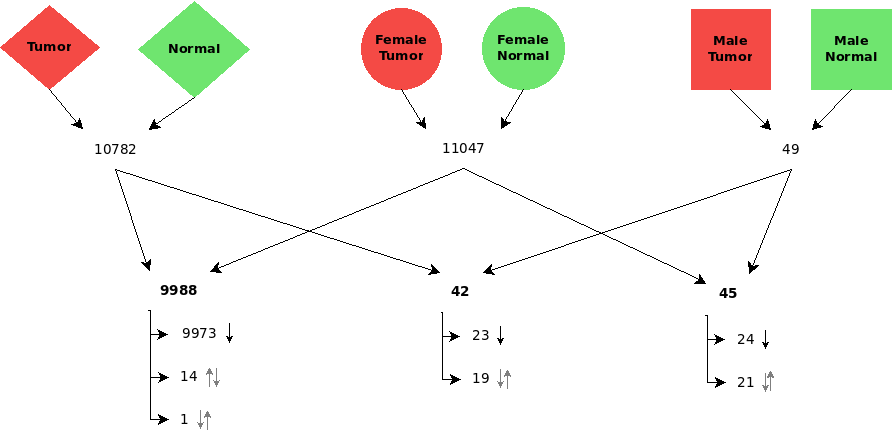
\includegraphics[width=\linewidth]{scheme}
\caption{Summary scheme of contrats made and their DE genes found on each}
\label{fig:scheme}
\end{figure}

\begin{figure}
\centering
\includegraphics[width=\linewidth]{../IEO_report_files/figure-html/volcanoplot-1}
\caption{Volcano plot comparing DE genes between all tumor and all normal samples. Criteria for significantly DE genes is represented by the red lines at 2 $log_{2}$ fold-change and 4.6  $log_{2}$ Odd ratio (99\% probability that the gene is differentially expressed between the the conditions being compared). Most significant DE genes are down-regulated (under-expressed).}
\label{fig:volcano1}
\end{figure}

\begin{figure}
\centering
\includegraphics[width=\linewidth]{../IEO_report_files/figure-html/volcano4-1}
\caption{Volcano plot comparing DE genes between female tumor samples and female normal samples. Criteria for significantly DE genes is represented by the red lines at 2 $log_{2}$ fold-change and 4.6 $log_{2}$ Odd ratio (99\% probability that the gene is differentially expressed between the the conditions being compared). Most significant DE genes are down-regulated (under-expressed).}
\label{fig:volcano2}
\end{figure}

\begin{figure}
\centering
\includegraphics[width=\linewidth]{../IEO_report_files/figure-html/volcano3-1}
\caption{Volcano plot comparing DE genes between male tumor samples and male normal samples. Criteria for significantly DE genes is represented by the red lines at 2 $log_{2}$ fold-change and 4.6 $log_{2}$ Odd ratio (99\% probability that the gene is differentially expressed between the the conditions being compared). Its pattern differs from the rest of the volcano plots because it has DE genes up regulated (over-expressed) as well as down regulated (under-expressed).}
\label{fig:volcano3}
\end{figure}

\begin{figure}
\centering
\includegraphics[width=\linewidth]{../IEO_report_files/figure-html/volcano2-1}
\caption{Volcano plot comparing DE genes between all male and all female samples. Criteria for significantly DE genes is represented by the red lines at 2 $log_{2}$ fold-change and 4.6 $log_{2}$ Odd ratio (99\% probability that the gene is differentially expressed between the the conditions being compared). Most significant DE genes are up-regulated (over-expressed).}
\label{fig:volcano4}
\end{figure}


We can see from the QQplots that DE genes from all comparisons differ from adjusting to a t-Student distribution (see Supplementary materials: Accuracy subsection). Furthermore, the volcano plots reveal an interesting extreme pattern in the comparisons between Tumor vs. Normal (see Figure \ref{fig:volcano1}) and Female-Tumor vs. Female-Normal (see Figure \ref{fig:volcano2}) where almost all DE expressed genes appear to be under-expressed. In contrast, the Male-Tumor vs. Male-Normal (see Figure \ref{fig:volcano3}) comparison present a less extreme volcano plot. Interestingly, in the comparison between Female vs. Male (see Figure \ref{fig:volcano4}) where the contrast is done by gender, without taking into account the sample type (tumor or normal), we see the opposite extreme pattern where it is shown an over-expression of almost all genes. This is due to the main contribution of normal samples to this comparison. We can infer a higher gene expression in Female-Normal compared to Male-Normal samples whereas Female-Tumor and Male-Tumor samples do not have significant differences in gene expression. 

Venn diagrams also help to explore the consistency of the obtained DE genes among the different comparisons. In Figure \ref{fig:venn1} we can see that from the set of DE genes between Tumor and Normal condition almost all (9988) of them are shared with females (Female-Tumor vs. Female-Normal). So, not only most of the DE genes are down-regulated (same pattern) in both comparisons but also almost all of them are shared. Additionally, in Table \ref{tab:1} we can see a summary of the number of DE expressed genes in the 3 comparisons that are more interesting for our analysis and the resulting genes from the intersection between the mentioned DE gene sets.


As a summary of our results:
\begin{itemize}
\item Female-Tumor = FT
\item Male-Tumor = MT
\item Female-Normal = FN
\item Male-Normal = MN
\end{itemize}

\bigskip

\begin{table*}[t]
  \centering
  \begin{tabular}{c|cccccccc}
     Regulation & FT Vs FN & MT Vs MN & FT Vs MT & FN Vs MN & T Vs N & F Vs M & FT Vs MN & FN Vs MT \\ \hline
     Down & 10845 & 42 & 3 & 1 & 10626 & 1 & 54 & 6 \\ 
     Not DE & 952 & 11721 & 11798 & 698 & 1147 & 689 & 11701 & 925 \\
     UP & 4 & 38 & 0 & 11102 & 28 & 11111 & 46 & 10870
  \end{tabular}
  \caption{Number of genes up-regulated, down-regulated and not differentially expressed genes in the different comparisons}
  \label{tab:1}
\end{table*}

                     
All in all, the fact that Female-Normal samples have more up-regulated DE genes respect to the rest of the samples (see Table \ref{tab:1}) 
is the key to understand our results and their patterns. From this comparisons we can see a pattern of how these interactions are related between them: it seems that the higher interaction is due to being a female, rather than having a specific development of the cancer on females or in males, or being male. The relationship between the interaction of factors can be expressed as $FT \approx MT \approx MN < FN$.

For further investigation, we have also performed a functional enrichment analysis with the sets of DE genes that where more interesting in order to elucidate the mechanisms that are altered in thyroid tumoral processes. In the case of DE expressed genes between Tumor and Normal samples we obtained several GO terms  % GO_tumor_table.html
related to regulation of metal ions, and acid and lipids regulation, like high-density lipoprotein particle assembly and very-low-density lipoprotein particle remodeling, as well as phosphorilation and ERK1 and ERK2 cascade, cardiac conduction system development, regulation of apoptotic DNA fragmentation among many others. This genes ontologies reflect the same behavior as in the comparison of between tumoral and normal females samples. % GO_female_table.html 
However, in that case other specific processes related with DNA damage response that include the well-known p53 pathway appear together with cell adhesion processes (either to other cells or to the matrix), chemotaxis related processes and migration of vascular and immune response cells. 
%GO_tumor_females_down_table-1.html
As we could expect, this processes also appear when taking the gene set shared by tumor vs. normal samples and female tumor vs. female normal samples. 
	 	
% GO_gender_table.html & DE_gender
Looking in the comparison between females and males there is a predominance of GO terms related to movement like motor neuron axon guidance and positive chemotaxis, followed by ion metal transport. Surprisingly the GO term with the lowest p-value and highest OddsRatio is related to the regulation of cholesterol transport, confirming the high requirements of energy of the tumor, specially in women. One special enriched GO is positive thymic T cell selection, with higher restriction on which T-cell are selected, the tumor in females might be able to develop earlier and stronger in females than in males. The most expressed gene in this comparison is DDX42, among its related pathways are mRNA Splicing and GO annotations relate it with nucleic acid binding and ATP-dependent RNA helicase activity.

% DE_males, GO_males_exc, GO_males
However the differentially expressed genes in the comparison Male-Tumor vs Male-Normal, are related to regulation of transcription, DNA-templated and regulation of several process as macromolecule metabolic process, biological quality, primary metabolic process. (See Supplementary GO tables)

% Summary of GO interpretation by Mauro, translated by Lluís
In general we can see that the interaction of gender with the tumor in women affects to the function of the cells. As they lose the capacity to perform they specific task they gain capacity to become tumoral. Some of the unexpected GO terms found could be due to parathyroid cells in the original samples, which are known to be in different regions depending on the person, who could be taken in the sample.

%La gran flipada de la Inés
\textbf{In light of the results, we suggest the following hypothesis. It is well known that lipid metabolism is more active in women than men as there is more fatty tissue respect to the whole body in females than males \citep{Blaak2001}. Therefore, by default we could expect that those genes are more DE expressed in females than males as we have found that there are more DE genes in female normal samples than any other type of sample. Some of the DE genes that we have found in our study are genes related to lipid metabolism specifically in females. Therefore, we could think that a down regulation of some of the genes of the lipid pathways are favouring the female tumorgenesis access to more fatty acids and therefore an earlier appearance and stronger tumors in females than males. As a consequence, this might be the reason why we find more Papillary Thyroid Carcinoma in females than males. Further investigation must be done in order to confirm our suspicion so our results must be taken with caution.}
 
\begin{figure}
\centering
\includegraphics[width=\linewidth]{../IEO_report_files/figure-html/venn_plots-1}
\caption{Venn diagram that shows DE genes shared between Tumor vs. Normal condition and Tumor-Female vs- Normal-female condition }.
\label{fig:venn1}
\end{figure}

  
\bibliography{IEO}

\end{document}
